As realizações desse período incluem simulações para a análise dos efeitos da hidrodinâmica realista em observáveis de jatos. Vários observáveis de estrutura a forma de jatos foram analizados, bem como observáveis relativos à correlação do jato com o meio hidrodinâmico produzido em colisões de íons pesados. Também nesse período trabalhei em monitorias das disciplinas de Física Experimental III e IV. Além disso, compareci ao XL Encontro Nacional de Física de Partículas e Campos, onde apresentei alguns resultados obtidos nesse trabalho. O mais relevante destes é a análise do observável $v_2$, que mede a assimetria anisotrópica azimutal, esse resultado pode ser visto na Figura \ref{v2}. Como se pode observar, ainda não há concordância experimental a respeito da magnitude dessa anisotropia, mas há concordância a respeito do fato de que ela existe, isso é suportado por outros observáveis que indicam flutuações significativas nas condições iniciais. O trabalho mostra que a inclusão de hidrodinâmica mais realista aliada a condições iniciais também mais realistas conseguem reproduzir essa assimetria diferente de zero. É importante salientar que a magnitude ainda precisa ser estudada com mais cuidado, assim como a dependência com o momento transversal.

\begin{figure}
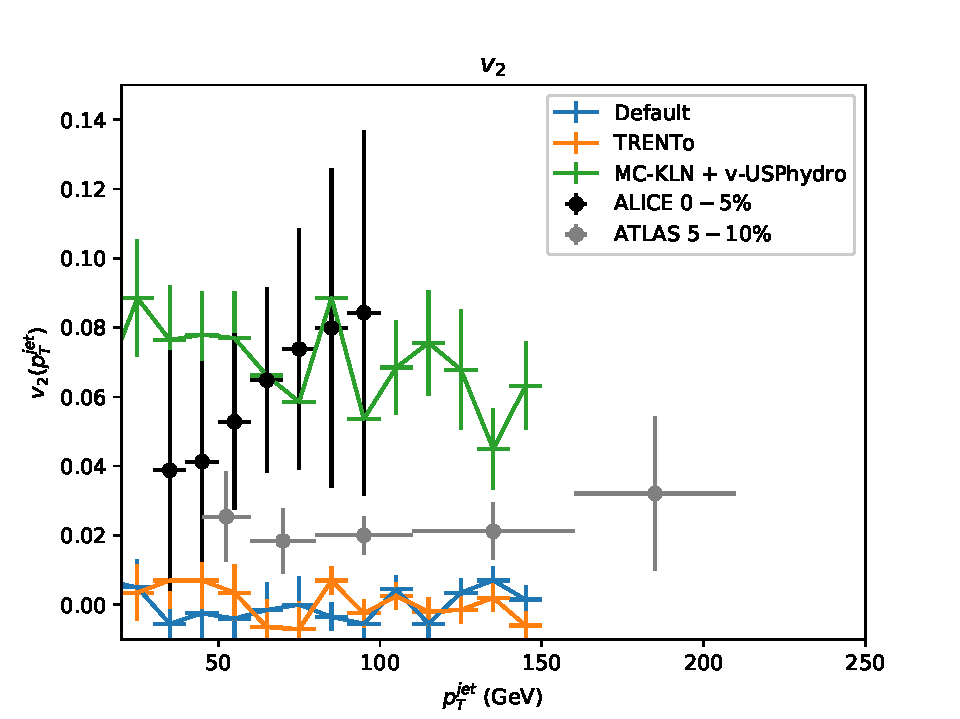
\includegraphics[width=1\textwidth]{Images/v2_5-eps-converted-to.pdf}
\caption{Análise da assimetria anisotrópica azimutal.}
\label{v2}
\end{figure}